% Created 2015-11-03 Tue 20:51
\documentclass[11pt]{article}
\usepackage[utf8]{inputenc}
\usepackage[T1]{fontenc}
\usepackage{fixltx2e}
\usepackage{graphicx}
\usepackage{grffile}
\usepackage{longtable}
\usepackage{wrapfig}
\usepackage{rotating}
\usepackage[normalem]{ulem}
\usepackage{amsmath}
\usepackage{textcomp}
\usepackage{amssymb}
\usepackage{capt-of}
\usepackage{hyperref}
\usepackage{minted}
\usepackage{minted}
\usemintedstyle{emacs}
\usepackage[spanish]{babel}
\addto{\captionsspanish}{\renewcommand*{\contentsname}{Contenido}}
\renewcommand{\listingscaption}{Código}
\date{}
\title{}
\hypersetup{
 pdfauthor={},
 pdftitle={},
 pdfkeywords={},
 pdfsubject={},
 pdfcreator={Emacs 24.5.1 (Org mode 8.3.1)},
 pdflang={Spanish}}
\begin{document}

\newcommand{\set}[2]{\newcommand{#1}{#2}}
\newcommand{\materia}[1]{\set{\Cmateria}{#1}}
\newcommand{\tipo}[1]{\set{\Ctipo}{#1}}
\newcommand{\titulo}[1]{\set{\Ctitulo}{#1}}
\newcommand{\resumen}[1]{\set{\Cresumen}{#1}}
\tipo{Apuntes}
\titulo{}
\materia{Redes de circuitos eléctricos}
\set{\logoDeLaUniversidad}{/home/hao/dev/org/latex-plantilla/figures/UDG.png}
\set{\largoDelLogo}{7cm}
\set{\nombreDeLaUniversidad}{Universidad de Guadalajara}
\set{\nombreDelDepartamento}{Departamento de electrónica}
\set{\nombreDelAutor}{Eduardo Vazquez Diaz}
\set{\emailDelAutor}{lalohao@gmail.com}
\title{
  \textbf{\nombreDeLaUniversidad}\\
  \nombreDelDepartamento\\
  \begin{figure}[ht]
    \centering
    \includegraphics[width=\largoDelLogo]{\logoDeLaUniversidad}
  \end{figure}
  \textbf{\Ctipo{}}\\
  \Ctitulo{}\\
  \textit{\Cmateria{}}\\
}
\author{\nombreDelAutor{}\\\emailDelAutor{}}
\maketitle
\newpage
\tableofcontents
\newpage
\ifdef{\Cresumen}{
\begin{abstract}
  \Cresumen{}
\end{abstract}
}{}

\section{Metodología}
\label{sec:orgheadline3}
\subsection{Evaluacion}
\label{sec:orgheadline1}
\begin{itemize}
\item 60\% examen
\begin{itemize}
\item 30\% examen
\item 30\% examen
\end{itemize}
\item 40\% tareas/actividades
\end{itemize}
\subsection{Libro}
\label{sec:orgheadline2}
Analisis de circuitos en ingenieria
William Hayt
\newpage
\section{Circuitos polifásicos}
\label{sec:orgheadline8}
\subsection{Sistemas monofásicos de 3 hilos balanceado}
\label{sec:orgheadline4}
\begin{wrapfigure}{r}{0.4\textwidth}
\centering
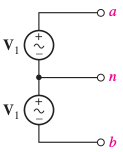
\includegraphics[width=4cm]{data/8e/bfa3bf-b466-4403-8824-a12d81b26121/screenshot-20151103-204646.png}
\caption{Diagrama de un sistema monofasico de 3 hilos}
\end{wrapfigure}

Son aquellos sistemas en el cual la fuente tiene 3 hilos y las
mediciones del voltimetro muestran la presencia de tensiones
senoidales de igual amplitud entre dos terminales cualesquiera.

$$V_{an}=V_{nb}$$
por lo que:
$$V_{ab}=V_{an}+V_{nb}=2V_{an}=2V_{nb}$$
$$$$$$$$$$$$

\begin{wrapfigure}{l}{0.4\textwidth}
\centering
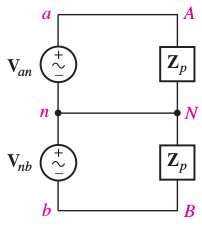
\includegraphics[width=4cm]{data/8e/bfa3bf-b466-4403-8824-a12d81b26121/screenshot-20151021-015512.png}
\caption{Sistema con cargas balanceadas}
\end{wrapfigure}

Cuando se conectan dos cargas (impedancias) idénticas las corrientes
también son idénticas:
$$I_{aA}=\frac{V_{an}}{Z_p}=I_{Bb}=\frac{V_{ab}}{Z_{p}}$$

Aplicando L.C.K en el \emph{neutro} (nodo \(nN\)) se obtiene una
característica fundamental de los circuitos polifásicos balanceados:
$$I_{nN}=I_{Bb}+I_{Aa}=I_{Bb}-I_{aA}=0$$

Lo que significa que no fluye corriente por el neutro.
\newpage
\subsection{Comparación de cargas trifásicas conectadas en Y y \(\Delta\)}
\label{sec:orgheadline5}
\begin{table}[htb]
\caption{Comparación de voltaje y corriente}
\centering
\begin{tabular}{lllll}
Carga & Tension de fase & Tension de linea & Corriente de fase & Corriente de linea\\
\hline
Y & \(V_{AN}=V_p\angle\theta\) & \(V_{AB}=\sqrt{3}V_p\angle\theta +30\) & \(I_{aA}=I_{AN}=\frac{V_{AN}}{Z_p}\) & ''\\
 & \(V_{BN}=V_p\angle\theta -120\) & \(V_{BC}=\sqrt{3}V_p\angle\theta -90\) & \(I_{bB}=I_{BN}=\frac{V_{BN}}{Z_p}\) & ''\\
 & \(V_{CN}=V_p\angle\theta -240\) & \(V_{CA}=\sqrt{3}V_p\angle\theta -210\) & \(I_{cC}=I_{CN}=\frac{V_{CN}}{Z_p}\) & ''\\
\hline
\(\Delta\) & \(V_{AB}=\sqrt{3}V_p\angle\theta\) & '' & \(I_{AB}=\frac{V_{AB}}{Z_p}\) & \(I_{aA}=(\sqrt{3}\angle\theta)\frac{V_{AB}}{Z_p}\)\\
 & \(V_{BC}=\sqrt{3}V_p\angle\theta -120\) & '' & \(I_{BC}=\frac{V_{BC}}{Z_p}\) & \(I_{bB}=(\sqrt{3}\angle\theta)\frac{V_{BC}}{Z_p}\)\\
 & \(V_{CA}=\sqrt{3}V_p\angle\theta -240\) & '' & \(I_{CA}=\frac{V_{CA}}{Z_p}\) & \(I_{cC}=(\sqrt{3}\angle\theta)\frac{V_{CA}}{Z_p}\)\\
 &  &  &  & \\
\end{tabular}
\end{table}

\begin{table}[htb]
\caption{Comparación de potencia}
\centering
\begin{tabular}{ll}
Carga & Potencia por fase\\
\hline
Y & \(\sqrt{3}V_LI_Lcos\theta\)\\
\(\Delta\) & \(\sqrt{3}V_LI_Lcos\theta\)\\
\end{tabular}
\end{table}

donde \(\cos\theta\) es el factor de potencia de la carga
\newpage
\subsection{Análisis del desplazamiento del neutro en conexión estrella balanceada}
\label{sec:orgheadline7}
\begin{figure}[htb]
\centering
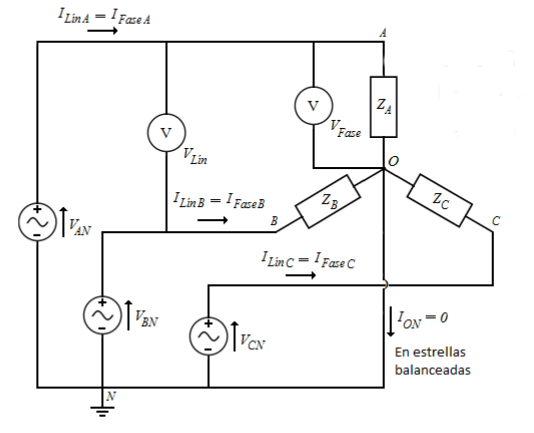
\includegraphics[width=.9\linewidth]{data/b3/9c0d3b-9738-4e7a-9ce8-bee35cfe403a/screenshot-20151103-204729.png}
\caption{Diagrama de fuentes en estrella conectado a cargas en estrella. Tambien conocido como Y-Y.}
\end{figure}

$$V_{AN}=\frac{V_{LinA}}{\sqrt{3}};I_{LinA}=\frac{V_{LinA}}{Z_{A}}$$
\begin{equation}\label{eq:voltaje-desbalanceado}
V_{AO}=V_{AN}+V_{NO}=V_{AN}-V_{ON}
\end{equation}
$$\therefore V_{BO}=V_{BN}-V_{ON}$$
$$\therefore V_{CO}=V_{CN}-V_{ON}$$

Aplicando L.C.K. al nodo \(N\).
$$I_{AO}+I_{BO}+I_{CO}=0$$
$$\frac{V_{AO}}{Z_A}+\frac{V_{BO}}{Z_B}+\frac{V_{CO}}{Z_C}=0$$
\begin{equation}\label{eq:lck-desbalanceado}
V_{AO}Y_A + V_{BO}Y_B  + V_{CO}Y_C=0
\end{equation}

Cuando la tierra fisica no esta conectada, y \(Z_A\), \(Z_B\), \(Z_C\)
son cargas diferentes se crea un voltaje \(V_{ON}\), si este
voltaje es mayor a la norma entonces el circuito se desbalancea.

Sustituyendo las ecuaciones (\ref{eq:voltaje-desbalanceado}) en la
ecuación (\ref{eq:lck-desbalanceado}):
$$ (V_{AN}-V_{ON}) Y_A+ (V_{BN}-V_{ON}) Y_B+ (V_{CN}-V_{ON}) Y_C=0$$
$$ V_{AN}Y_A + V_{BN}Y_B + V_{CN}Y_C=V_{ON}(Y_A+Y_B+Y_C)$$
\begin{equation}\label{eq:voltaje-neutro}
V_{ON}=\frac{V_{AN}Y_A + V_{BN}Y_B + V_{CN}Y_C}{Y_A+Y_B+Y_C}
\end{equation}

La ecuación (\ref{eq:voltaje-neutro}) describe el voltaje en el
neutro a causa de un desbalance.
\subsubsection{Ejemplo}
\label{sec:orgheadline6}
Una conexion estrella desbalanceada cuyas impedancias son:
\(Z_A=12\angle 0\), \(Z_B=8\angle 45\), \(Z_C=10\angle 30\) (en grados)
se alimenta con un sistema trifasico de 4 hilos cuyo voltaje de
linea es \(220v\) secuencia \(ABC\) .
\begin{enumerate}
\item Calcule el valor de cada corriente de linea.
\item La corriente que circula del neutro a tierra.
\item La potencia aparente que consume cada fase y la potencia
aparente total.
\end{enumerate}

$$(1)$$
$$I_{LinA}= 13.018046815794099\angle-6.686239852427747$$
$$I_{LinB}= 16.622401736597524\angle-150.4259528457764$$
$$I_{LinC}= 9.838937778497865\angle81.06982369527327$$
$$(2)$$
$$I_N=8.358438485664404e-15<39.61068824002659$$
\section{Inductancia mutua}
\label{sec:orgheadline11}
\begin{wrapfigure}{l}{0.5\textwidth}
\centering
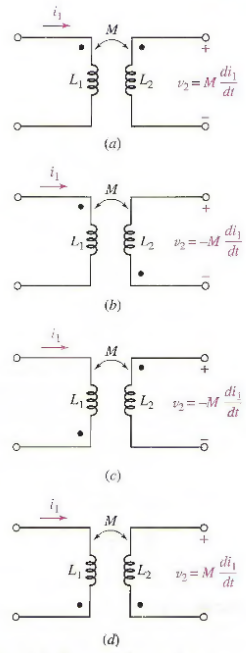
\includegraphics[width=6cm]{data/e4/817abd-f3f7-4574-aada-b974440e3a0e/screenshot-20151103-204815.png}
\caption{Convención del punto}
\end{wrapfigure}

El voltaje en un inductor esta dado por:
$$v(t)=L \frac{di}{dt}$$

Cuando el voltaje esta siendo inducido por otro inductor como en el
caso de los transformadores el voltaje se vuelve:
$$v(t)=\pm M \frac{di_2}{dt}$$

Donde \(M\) es el coeficiente de inductancia, y el signo de la
corriente se determina por medio de la convención del punto.
\subsection{Ejemplo 1}
\label{sec:orgheadline9}
La ecuación (\ref{eq:convencion-punto}) describe el voltaje en el
inductor \(2\) producido por el inductor \(1\) suponiendo que la
convención del punto sea determinada por la figura (a).
\begin{equation}\label{eq:convencion-punto}
V_2=M_{21}\frac{di_1(t)}{dt}
\end{equation}

Cuando se aplica un voltaje también en \(V_2\) la ecuación se vuelve:
$$V_2=L \frac{di_2}{dt}+M\frac{di_1}{dt}$$
$$$$

\subsection{Ejemplo 2}
\label{sec:orgheadline10}
\begin{wrapfigure}{r}{0.3\textwidth}
\centering
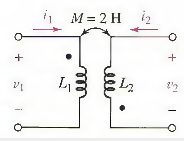
\includegraphics[width=4cm]{data/f4/1900ab-403b-4c90-9cf4-f6dd53803938/screenshot-20151103-204917.png}
\end{wrapfigure}

En el siguiente circuito determina (a) \(v_1\) si \(i_2=5\sin{45t}A\) e
\(i_1=0\); (b) \(v_2\) si \(i_1=-8e^{-t}A\) e \(i_2=0\)
$$(a)v_1=- (2) (45) (5 \cos{45t})=-450 \cos{45t} $$
$$(b)v_2=- (2) (-1) (-8 e^{-t})=-16e^{-t} $$

\section{Frecuencia compleja}
\label{sec:orgheadline15}
En el dominio de \(s\) es posible analizar algunos aspectos de los
circuitos de una forma mas sencilla comparado al uso de ecuaciones
diferenciales.
$$s=\alpha+j\omega$$

Partiendo de una función de voltaje real \(v(t)=V_m e^{\sigma t} \cos{(\omega t+\theta)}\),
utilizando la idendidad de euler se obtiene
$$v(t)=f(t)=Ke^{st}$$

De la cual se pueden deducir los siguientes casos:
\begin{itemize}
\item Corriente Directa (CD)
\item Exponencial
\item Senoidal
\item Senoidal amortiguado exponencialmente
\end{itemize}

\subsection{Caso CD}
\label{sec:orgheadline12}

\subsection{Caso seno amortiguado exponencialmente}
\label{sec:orgheadline14}
$$v(t)=Re \left\{V_m e^{\sigma t} e^{j (\omega t +\theta)}  \right\}$$
$$v(t)=Re \left\{V_m e^{j\theta} e^{st}  \right\}$$


$$\frac{1}{2} V_m e^{j\theta} e^{(\sigma + j\omega)t} + \frac{1}{2} V_m e^{-j\theta} e^{(\sigma - j\omega)t}$$
\subsubsection{Ejemplo}
\label{sec:orgheadline13}
\begin{verbatim}
Convertir a forma general
(a) s=7+j0
(b) s=0+j10
\end{verbatim}
$$(1)Ke^{7t}$$
$$(2)Ke^{j10t}=K \left[ cos(10t)-jsen(10t) \right] $$

\begin{verbatim}
Identifique las frecuencias complejas de la siguiente ecuacion:
\end{verbatim}
\((2 e^{-100t}+ e^{200t}) \sin{2000t}\)
$$2 e^{-100t} \sin{2000t} +e^{200t}\sin{2000t} $$
$$\therefore s_1=-100\pm 2000;s_2=200\pm 2000$$
Aplicar la funcion forzada \(v(t)=60 e^{-2t} \cos{4t+10}\) al
circuito RLC de la figura y especificar la respuesta forzada
determinando \(I_m\) y \(\phi\) en la expresion \(i(t)=I_m e^{-2t} \cos{4t+\phi}\)

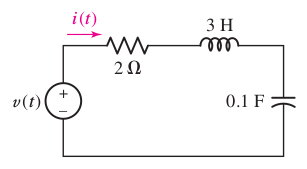
\includegraphics[width=6cm]{data/3d/2b2155-c4a3-4377-9dc1-c7656ef5dd8c/screenshot-20151013-181600.png}

$$v(t)=60 e^{-2t} \cos{4t+10} = Re \left\{ 60 e^{-2t} e^{j (4t+10)} \right\}=Re \left\{ 60 e^{j10} e^{(-2+j4)t} \right\}$$
$$V=60\angle 10;s=-2+j4$$
\section{Transformada de Laplace}
\label{sec:orgheadline26}
$$\mathcal{L}\left\{ te^{-\alpha t}u(t) \right\}=\frac{1}{(s+\alpha)^2}$$
\subsection{Bilateral}
\label{sec:orgheadline16}
$$F(s)=\int\limits_{-\infty}^{\infty} e^{-st} f (t)dt $$
\subsection{Unilateral}
\label{sec:orgheadline17}
$$F(s)=\int\limits_{0}^{\infty} e^{-st} f (t)dt $$
\subsection{Ejemplo}
\label{sec:orgheadline18}
Obtener la transformada de Laplace unilateral para \(f(t)\)
$$f (t)=2u (t-3)$$
$$F (s)=\int\limits_{0^-}^{\infty} e^{-st} 2u (t-3)dt=2\int\limits_{3}^{\infty} e^{-st}dt=-\frac{2}{s} e^{-st}\bigg|^{t=\infty}_{t=3}$$
$$F (s)=-\frac{2}{s} (e^{-\infty s}-e^{-3 s})=-\frac{2}{s} (- e^{-3s})=\frac{2e^{-3s}}{s}$$

Obtener la transformada de Laplace unilateral
$$f (t)=u(t)$$
$$F (s)=\int\limits_0^{\infty}e^{-st}dt=-\frac{e^{-st}}{s}\bigg|^{\infty}_0=-\frac{1}{s} (e^{-\infty s}-e^{-0s}) =-\frac{1}{s} (-e^0)=\frac{1}{s} $$

Obtener la transformada de Laplace unilateral
$$f (t)=-6e^{-2t}\left[ u (t+3)-u (t-2) \right] $$
\subsection{Impulso unitario}
\label{sec:orgheadline19}
\subsection{Teorema de la linealidad}
\label{sec:orgheadline20}
$$\mathcal{L}\left\{ f_1(t)+f_2(t) \right\}=\int\limits_{0^-}^{\infty}e^{-st}\left[ f_1(t)+f_2(t) \right]dt=\int\limits_{0^-}^{\infty}e^{-st}f_1(t)dt+\int\limits_{0^-}^{\infty}e^{-st}f_2(t)dt=F_1(s)+F_2(s)$$
\subsection{Anti-transformada de Laplace}
\label{sec:orgheadline22}
$$V(s)\rightarrow v(t)$$
$$V(s)=V_1(s)+V_2(s)$$
$$v(t)=\mathcal{L}^{-1}\left\{ V(s) \right\}=\mathcal{L}^{-1}\left\{ V_1(s) + V_2(s)\right\}=\mathcal{L}^{-1}\left\{ V_1(s)\right\}+\mathcal{L}^{-1}\left\{V_2(s)\right\}$$
\subsubsection{Ejemplo}
\label{sec:orgheadline21}
Encontrar \(G(t)\)
$$G(s)=\frac{7}{s}-\frac{31}{s+17}$$
$$g(t)=\mathcal{L}^{-1}\left\{\frac{7}{s} \right\}-\mathcal{L}^{-1}\left\{\frac{31}{s+17}\right\}$$
$$g(t)=7u(t)-31e^{-17t}u(t)$$
$$g(t)=\left( 7-31e^{-17t} \right)u(t)$$

Dada la funcion \(H(s)=\frac{7}{s^2}+\frac{31}{(s+17)^2}\)
encontrar \(h(t)\)
$$h(t)=\mathcal{L}^{-1}\left\{\frac{7}{s^2}+\frac{31}{(s+17)^2}\right\}=(7+31e^{-17t})tu(t)$$
\subsection{Transformada inversa de funciones racionales}
\label{sec:orgheadline25}
\(P(s)=\frac{N(s)}{D(s)}\) donde \(N(s)\) y \(D(s)\) son polinomios.

Los valores de \(s\) que originan \(N(s)=0\) se conocen como
\textbf{ceros}.

Los valores de \(s\) que originan \(D(s)=0\) se conocen como
\textbf{polos}.
\subsubsection{Ejemplo}
\label{sec:orgheadline23}
Encontrar la transformada inversa de \(F(s)=2 \frac{s+2}{s}\)
$$F(s)=\frac{2s+4}{s}=2+\frac{4}{s}$$
$$f(t)=2\delta (t)+4u(t)$$

Dada \(Q(s)=\frac{3s^2-4}{s^2}\) encontrar \(q(t)\)
$$Q(s)=\frac{3s^2-4}{s^2}=3-\frac{4}{s^{2}}$$
$$q(t)=3\delta (t)-4tu(t)$$
\subsubsection{Polos distintos}
\label{sec:orgheadline24}
Encontrar transformada inversa de:
$$P(s)=\frac{7s+5}{s^2+s}=\frac{7s+5}{s(s+1)}=\frac{A}{s}+\frac{B}{s+1}$$
$$A=\frac{7s+5}{s+1}\bigg|_{s=0}=5$$
$$B=\frac{7s+5}{s}\bigg|_{s=-1}=2$$
$$\therefore P(s)=\frac{5}{s}+\frac{2}{s+1}$$
$$p(t)=5u(t)+2e^{-t}u(t)$$

Encontrar la transformada inversa de:
$$P(s)=\frac{11s+30}{s^2+3s}=\frac{11s+30}{s(s+3)}$$
$$A=\frac{11s+30}{s+3}\bigg|_{s=0}=10$$
$$B=\frac{11s+30}{s}\bigg|_{s=-3}=$$
\end{document}
